\section{实验结果与分析}
% 一些关于序号的设置
\setcounter{figure}{0}

\subsection{改进SSD算法的实验结果}
\begin{uscfigure}
	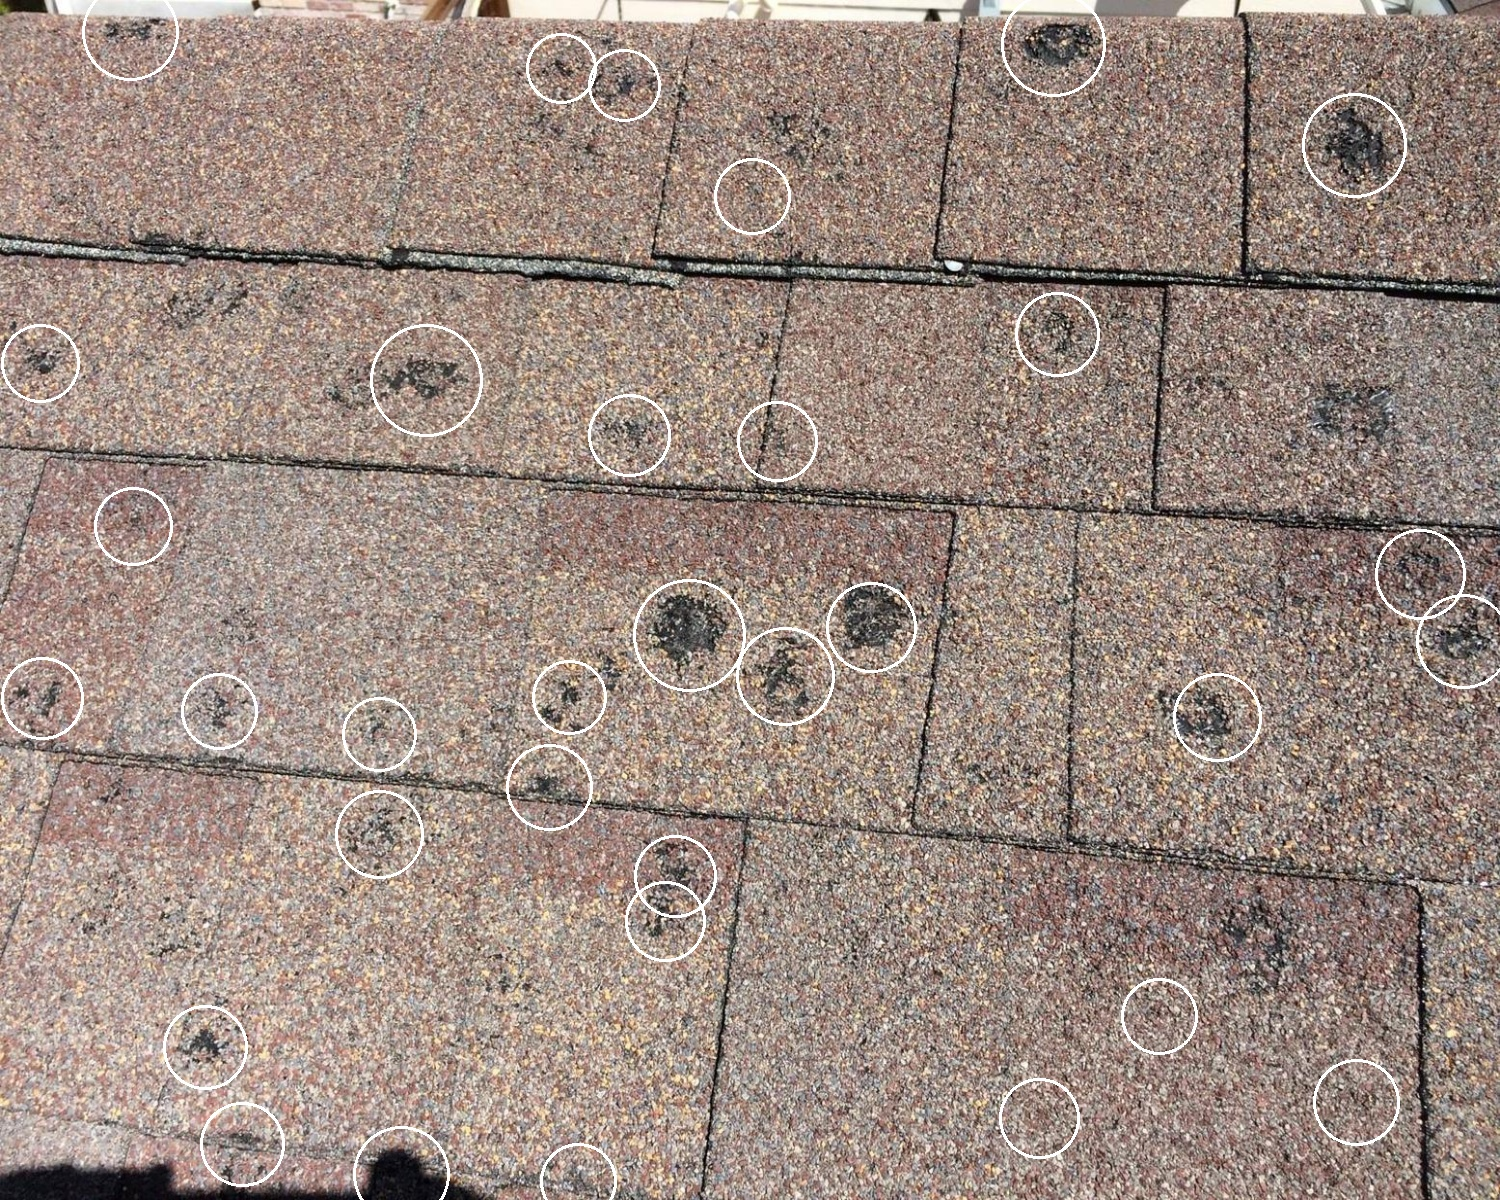
\includegraphics[width=\textwidth]{./Pictures/result.jpg}	
	\caption{检测结果}
	\label{result}
\end{uscfigure}

\subsection{改进SSD对瓦片损害检测的准确率实验}
\begin{table}[htbp]
	\centering
	\caption{改进SSD算法的准确率实验结果}
	\label{}
	\begin{tabular}{ccc}
		\toprule
		网络模型 & mAP & fps\\
		\midrule
		SSD 	& 60\% & 80\\
		改进SSD  &  65\% & 80\\
		\bottomrule
	\end{tabular}
\end{table}
\subsection{实验结果分析}
从瓦片损害的检测实验过程中发现,其结果是低于原算法在PACSL VOC数据库中的实验结果的,其具体原因和以下几点:

1、瓦片损害的形态不定,且与距离受损害的时间的长短有关——时间越长损害处的颜色越深,不利于标注从而导致降低了算法的识别精度。

2、数据量不够导致了降低了识别精度,由于没有现成的房屋屋顶瓦片数据,且一般家庭住房不愿意无人机拍照。

3、相当数量的房屋屋顶年代久远,以至于瓦片自身已经风化,为检测任务添加了不确定性
\begin{uscfigure}
	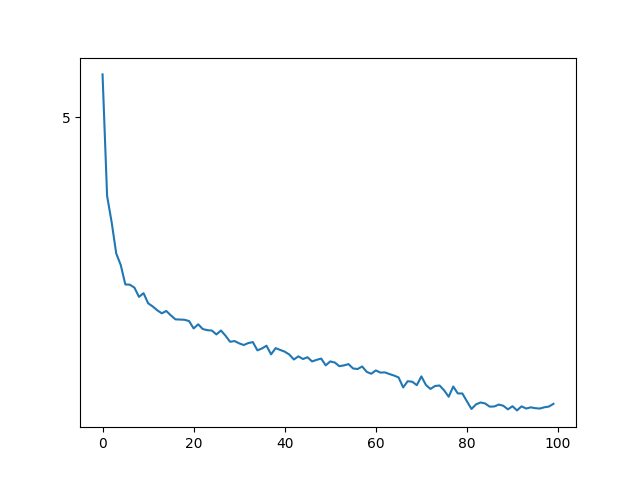
\includegraphics[width=\textwidth]{./Pictures/loss.png}	
	\caption{梯度下降图}
	\label{result}
\end{uscfigure}
\subsection{算法改进建议}
随着目标识别相关算法的成熟,现在的识别精度已经超过了80\%,房屋瓦片损害检测只能充分利用其自身的特点,手工设计一些特征,从而提高算法的识别精度。与此同时,数据量是一个急需解决的问题,数据量一大,对于一些干扰就能有效的去除。
